

\documentclass{article}
\usepackage[utf8]{inputenc}
\usepackage{authblk}
\usepackage{setspace}
\usepackage{natbib}
\usepackage{hyperref}
%\usepackage{cite}
\usepackage[margin=1in]{geometry}
\usepackage{array}
\usepackage{graphicx}
\usepackage{caption}
\graphicspath{ {./figures/} }
\usepackage{subcaption}
\usepackage{amsmath}
\usepackage{lineno}
\usepackage{soul}
\usepackage{xcolor}
\sethlcolor{yellow}
\linenumbers

%%%%%%%%%%%%%%%%%
\title{Thesis Proposal}
\date{\today}
\author{Christophe Rouleau-Desrochers}

\begin{document}
%%%%%%%%%%%%%%%%%%%%%%%%%%%%%%

\maketitle


%<><><><><><><><><><><><><><><><><><><><><><><><><><><><><><><><><><><><><><><><>
% INTRODUCTION %
%<><><><><><><><><><><><><><><><><><><><><><><><><><><><><><><><><><><><><><><><>
\section{Introduction}
% <><><><><><><><><><><><><><><><><><><><><><><><><><><><><><>
% SECTION 1.1. %
% <><><><><><><><><><><><><><><><><><><><><><><><><><><><><><>
\subsection{Climate change impacts on tree phenology}
Research from the past decades has shown convincing evidence that human activity is increasingly affecting many worldwide environmental processes \citep{ceballos_biological_2017,intergovernmental_panel_on_climate_change_ipcc_climate_2023,laurance_have_2007,parmesan_globally_2003}. This can be through land use change and destruction, pollution, invasive species, resource overexploitation and climate change \citep{driscoll_biodiversity-crisis_2018,parmesan_poleward_1999,wu_key_2013}. That alone raises major concern, and actions have been deployed to mitigate these impacts, with varying success (e.g. \citep{campbell_producing_2014}). Even though immediate actions can have positive impacts and potentially reduce some threats to biodiversity, reversing 150 years of human-induced greenhouse gas emissions is harder. These emissions have affected Earth's climate and are projected to keep changing it for many centuries \citep{intergovernmental_panel_on_climate_change_ipcc_climate_2023}.
While there is a scientific consensus that observed climate change is human-caused \citep{intergovernmental_panel_on_climate_change_detection_2014,lynas_greater_2021,oreskes_scientific_2004}, the magnitude and the extent of the consequences that a warming climate will have on biological processes are still debatable \citep{huey_predicting_2012}. Historically, the first case of attribution of a biological change to climate change was on poleward shifts of European butterflies in Europe in response to regional warming \citep{parmesan_poleward_1999}. \\

% <><><><><><><><><><><><><><><><><><><><><><><><><><><><><><>

% <><><><><><><><><><><><><><><><><><><><><><><><><><><><><><>
\textbf{1.1.2. Trends of spring and autumn phenological events and their drivers} \\ 
The most frequently observed biological impact of climate change over the past decades is major changes in spring and autumn phenology                                                                                                                                                                                                                                                                                                                                                                                                                                                 ---the timing of recurring life history events \citep{parmesan_globally_2003,cleland_shifting_2007,lieth_phenology_1974,woolway_phenological_2021,menzel_european_2006}. Understanding the consequences of these shifts on ecosystems requires understanding how much the growing season has changed \citep{duputie_phenological_2015}. Spring phenological events (e.g. budburst and leafout) have been advancing from 0.5 \citep{wolfe_climate_2005} to 4.2 days/decade \citep{chmielewski_response_2001,fu_recent_2014} and are mainly driven by temperature \citep{chuine_why_2010,cleland_shifting_2007,penuelas_responses_2001}. In contrast, autumn phenology (e.g. budset and leaf senescence) is delayed, though to a much lesser extent than spring \citep{gallinat_autumn_2015,jeong_macroscale_2014}. The drivers regulating autumn phenology are far less understood than those of spring for many reasons. First, autumn phenology has attracted much less attention compared to spring \citep{piao_plant_2019}. Second, the data is often much noisier, since meteorological conditions in the fall can drastically influence phenological phenomena. To illustrate this, trees going through leaf senescence are subjected to a gradual leaf abscission that follows nutrient reabsorption, and the leaves within the same individual might be at different senescence stages, but a strong wind spell may trigger leaf drop for all leaves, thus affecting the temporal resolution of these data \citep{wu_canopy_2024}. However, there is a general belief that autumn phenophases are driven by shortening photoperiod and colder temperatures \citep{cooke_dynamic_2012,flynn_temperature_2018,korner_phenology_2010,delpierre_temperate_2016}. Different hypotheses are proposed to explain delayed autumn phenophases. First, warmer autumn temperatures may extend the activity of photosynthetic enzymes, which could be maintained at a higher level. Thus, the degradation rate of chlorophyll would decrease and the timing of senescence would be delayed \citep{yan_divergent_2021}. Second, summer droughts could make trees pause their activity schedule and delay senescence to increase carbon assimilation \citep{dox_severe_2022}. Third, there could be an antagonistic effect of warming and brightening---caused by reductions in atmospheric pollution and cloud cover \citep{sanchezlorenzo_reassessment_2015}---on leaf senescence \citep{wu_atmospheric_2021}. Brightening accelerates the leaf senescence processes and reduces the temperature sensitivity during that period, counteracting the expected warming-induced delays in leaf senescence \citep{wu_atmospheric_2021}. The photo-protection and sink limitation hypotheses provide plausible explanations for the negative effect of radiation on leaf senescence and the declining effect of temperature sensitivity of leaf senescence in response to brightening \citep{wu_atmospheric_2021, zani_increased_2020}. \\

% DO THIS: REVISE THE LAST SENTENCE OF THE ABOVE PARAGRAPH
% <><><><><><><><><><><><><><><><><><><><><><><><><><><><><><>
\textbf{1.1.3. Misleading evidence of declining sensitivity to warming} \\ 
While we have convincing proof that spring events advanced in the past decades, there is evidence that this might decelerate because of declining sensitivity to warming \citep{fu_declining_2015,meng_urban_2020}. The proposed mechanism is through the action of warmer winters on tree dormancy. In the fall, trees in boreal and temperate forests slowly enter dormancy, which is initiated with budset. During this phase, cold hardiness increases, which prepares the tree for the upcoming cold temperatures and prevents tissue damage. Then, the tree enters dormancy, during which a certain duration of cold temperatures (chilling)---with some interaction with photoperiod for some species---is necessary for the trees to be ready to accumulate forcing \citep{vitasse_interaction_2014}. In the late winter and early spring, they go through two forms of deacclimation before budburst \citep{vitasse_interaction_2014}. When deacclimation is reached, a certain amount of heat (forcing) is required to initiate budburst \citep{fu_declining_2015}. The argument of declining sensitivity appears here: heat requirement is met sooner in warm springs, but it's also negatively correlated with chilling \citep{fu_declining_2015,fu_sensitivity_2013, laube_chilling_2014}. However, it is this interaction between chilling and forcing requirements that determines the timing of leaf unfolding. In other words, a decrease in chilling accumulation is proposed to explain the observed weaker spring temperature sensitivities, where spring forcing loses its relative importance \citep{fu_declining_2015,meng_urban_2020,wolkovich_simple_2021}. However, a meta-analysis compiling 72 studies of 203 species suggests that declining sensitivities observed in Europe may be a statistical artifact of how these responses are calculated, thus casting doubt on this proposed trend \citep{ettinger_winter_2020}. This statistical artifact is explained to be caused by using linear models for calculating non-linear processes \citep{wolkovich_simple_2021}. \\

% <><><><><><><><><><><><><><><><><><><><><><><><><><><><><><>
\textbf{1.1.4. Mechanisms that could limit growth despite having a longer growing season} \\ 
Plants' seasonal activity has internal and external controls, both determined by environmental conditions \citep{wolkovich_why_2025}. Internal controls operate via autonomous clocks, activating genes and releasing hormones which often rely on chilling and/or photoperiod \citep{korner_four_2023}. The external controls, often referred to as forcing, act directly on the developmental rate, meristem activity, tissue differentiation and metabolism \citep{korner_four_2023}. Understanding how these controls operate is critical to our comprehension of plants' capacity to adjust their activity schedule in response to changing conditions \citep{chuine_process-based_2017}. In light of this, I hypothesize two possible drivers that could explain why a longer growing season might not lead to increased growth: external (environmental) \citep{kolar_response_2016} and internal \citep{zohner_effect_2023} constraints to growth \citep{wolkovich_why_2025}. \\

\textit{1.1.4.1. External constraints} \\ 
The complex nature of climate change makes predicting the external limits to growth hard to quantify at the individual level, as these drivers affect communities as a whole. However, drought, spring frost and heat waves are commonly mentioned as the main extreme events that could limit tree growth under climate change \citep{tyree_xylem_2002, choat_triggers_2018, li_widespread_2023,trenberth_global_2014,intergovernmental_panel_on_climate_change_detection_2014,chiang_evidence_2021,polgar_leafout_2011,reinmann_compensatory_2023}. Their definitions, respective mechanisms, global trend of occurence, consequences and differences among species are described in Tables 3.1. (Spring frosts), 3.2. (Droughts) and 3.3. (Heat waves). \\

\textit{1.1.4.2. Internal constraints} \\  
As for the internal constraints to growth, recent hypotheses propose that broadleaf deciduous tree species may be sink-saturated, such that longer growing seasons with more carbon fixation do not necessarily increase growth \citep{dow_warm_2022}. This one pathway is directly linked to the internal controls of plant growth, which are under strong genetic control. In addition to height and radial growth varying across species, these growth responses also vary by site \citep{silvestro_local_2023, aitken_time_2016}. Populations from higher altitude or latitude grow less under the same conditions than individuals from lower altitude or latitude \citep{way_photoperiod_2015}. This is further supported by phenological studies showing that growth cessation arrives earlier from populations of higher latitude, demonstrating local adaptation to potentially avoid fall frost, before nutrient uptake has finished \citep{aitken_time_2016,vitasse_ontogenic_2013,way_photoperiod_2015}. These trees rely on photoperiod cues for setting buds (stopping height growth) \citep{way_photoperiod_2015, soolanayakanahally_timing_2013}.  \\

Growth seasonality has huge consequences on annual growth, but this seasonality is also closely tied to the environmental conditions experienced by an individual. For instance, warming spring temperatures seem to positively affect growth, but recent evidence suggests a shift in this net positive effect near the summer solstice. Indeed \cite{zohner_effect_2023} found that warmer temperatures before the solstice advanced the onset of senescence, but it slowed the progression of leaf colouring when temperatures post-solstice were warmer. This further reinforces the importance of understanding how the timing of warmer conditions affects tree species. \\ 

% <><><><><><><><><><><><><><><><><><><><><><><><><><><><><><>
\textbf{1.1.5. How these shifts translate into effects on trees/forests is not clear - Pros and cons of early/late start/end of season} \\ 
Shifts in spring and autumn phenology support a long-lasting and intuitive assumption that earlier spring and delayed autumn events lead to longer seasons---and thus increased growth \citep{keenan_net_2014, stridbeck_partly_2022}. However, research from the past three years has cast doubt on this hypothesis \citep{dow_warm_2022,green_limits_2022,silvestro_longer_2023}. For instance, \citep{dow_warm_2022} showed that despite an earlier growth onset, neither growth rate nor overall annual increment was increased by longer seasons. This could substantially affect carbon-cycle model projections and thus feedbacks to future climate \citep{richardson_climate_2013,swidrak_comparing_2013}. Starting to grow earlier and stopping later both have pros and cons (Figure 1).

Understanding these findings requires answering why trees do not grow more despite longer growing seasons. While carbon allocation to above-ground biomass is one of the largest carbon sinks, how this carbon is allocated into wood is poorly understood. Indeed, the linear relationship assumption between wood growth and carbon assimilation is not well supported mechanistically and represents an important limitation of vegetation models \citep{cabon_cross-biome_2022}. Net primary production represents the difference between photosynthesis and plant respiration, but this commonly used metric completely omits the representation of growth processes. This is perhaps because of a long-lasting paradigm of source-limited photosynthesis. This has now been debunked with carbon fertilization experiments, supporting evidence that direct environmental constraints on growth may be stronger than those on photosynthesis \citep{friend_need_2019,parent_modelling_2010}. This opens up a new---poorly tested---temperature sensitivity relationship between cambial activity and photosynthesis. Growing evidence suggests that cambial activity may be more sensitive than photosynthesis to a range of environmental conditions, such as water and nutrient availability, and temperature \citep{cabon_cross-biome_2022,cabon_water_2020,muller_water_2011,peters_turgor_2021}. This demonstrates that carbon projection models that heavily rely on vegetation alone may mislead the amount of carbon sequestrated in our forests. \\

% <><><><><><><><><><><><><><><><><><><><><><><><><><><><><><>
\textbf{1.1.6. Growing season shifts and consequences on forest ecosystems and services} \\ 
Spring and fall phenological events are shifting with debatable consequences on tree growth. The sensitivity of cambial activity to water, temperature and nutrients has the potential to have far-reaching consequences given the hard-to-predict nature of future climate change, where any of these variables could vary from low to high amplitude \citep{almagro_longterm_2025,cabon_cross-biome_2022}. This expected asymmetry of future environmental changes makes understanding the internal and external limits to growth critical. Especially, the capacity to tease apart different biomes---as for example boreal vs tropical forests are expected to react differently (REF)---is critical and empirical data coming from experiments, but also from observations are paramount to predict the changes of forest carbon offset from human GHG emissions \citep{wolkovich_why_2025}.  

% <><><><><><><><><><><><><><><><><><><><><><><><><><><><><><>
% SECTION 1.2 %
% <><><><><><><><><><><><><><><><><><><><><><><><><><><><><><>
\subsection{Nature of the problem, and how to address it}

\textbf{1.2.1. Past phenological trends can help (or not) predict future phenological changes} \\ 
Observed phenological trends in the last decades cannot be used directly to extrapolate future phenological changes because: (1) the mechanisms guiding them aren't clear, and (2) phenological responses of trees to warming are very likely to be non-linear \citep{ettinger_winter_2020,fu_sensitivity_2013}. Indeed, accurate predictions require an in-depth, accurate mechanistic understanding of phenophases and their sensitivities to environmental drivers, especially to temperature and photoperiod \citep{fu_sensitivity_2013}. Therefore, the very foundation of the assumption that longer seasons increase growth may shift with future climate change. The well-observed advance in spring phenology may decellarate, and delayed fall phenology may shift towards earlier leaf senescence (through summer drought-induced growth cessation). \\

\textbf{1.2.2. The assumption that longer seasons lead to increased growth is called into question} \\ 
Recent work shows an absence of increased growth despite apparent better environmental conditions, thus casting doubt on a simple and intuitive positive relationship between growing season length and growth. This paradox further emphasizes the need to better understand the drivers regulating growth across biomes, but also how these drivers vary across the species within these biomes. Phenology varies greatly across species (e.g. closely related species tend to budburst at similar times under similar conditions) \citep{wolkovich_progress_2014}, but so does the relationship between growth and season length, which may explain the wide variation of this relationship within communities \citep{buckley_functional_2012}. This highlights another weakness of current carbon sequestration models that pool species together, which likely overpass important nuances in the growth responses that could be explained by species differences. This may mislead the future of forest carbon source-sink ratios \citep{green_limits_2022,cabon_cross-biome_2022}. To better understand how different species respond to warming, different strategies can be used. \\


First, experiments are paramount to robustly tease apart the external vs internal drivers (e.g. warmer springs from severe drought later in the season---a common co-occurring reality in natural environments) \citep{morin_changes_2010,primack_observations_2015}. However, experiments are most often performed on juvenile trees, which are critical for their role in forest regeneration projections, but their responses can hardly be translated to mature trees, which hold the overwhelming carbon biomass proportion of forests \citep{augspurger_differences_2003,silvestro_longer_2023,vitasse_ontogenic_2013}. \\

Second, leaf phenology through ground-based observations can provide valuable insights into the growth temporality trees that are not suitable for experimental trials. Since cambial and leaf phenology are closely linked to the other, having the more accessible leaf phenology data can act as a reliable proxy for the onset and end of tree growth. It is to say that knowing when leaves elongate and colour can guide when trees start and stop growing---fundamental metrics to determine the growing season length. Ground observations have the advantage of providing accurate data on phenological events for specific sites and species. Recently, the widespread use of smartphones has opened a whole new world of possible phenological monitoring through citizen scientists' records of data over much larger areas and for a wider range of species \citep{dickinson_current_2012,hufkens_monitoring_2019,piao_plant_2019}. While there are drawbacks to these observations (e.g. non-standard protocols, highly uneven spatiotemporal distribution of these observations), these methods have a huge potential to diversify the phenology data. \\

\textbf{1.2.3. Goals of my thesis}  \\ 
Using citizen science data, a common garden study and a large-scale experiment, I aim to better understand how different tree species, at different lifespan stages, vary in their growth responses to different season length. 

% <><><><><><><><><><><><><><><><><><><><><><><><><><><><><><>
% SECTION 1.3. %
% <><><><><><><><><><><><><><><><><><><><><><><><><><><><><><>
\subsection{Complexity of measuring growth and defining growing season length} 
\textit{1.3.1. What is a growing season?} \\
To understand how trees respond to growing season conditions, it is important to clarify what a growing season and growth are. \\
First, a problem that arises when one tries to quantify how shifting growing seasons affect growth comes from the definition of the growing season itself. Recently, \cite{korner_four_2023} proposed four definitions addressing this issue: (1) true growing season, based on measurable growth; (2) phenological season, based on visible phenological markers; (3) the productive season, based on primary production and (4) meteorological season, based on environmental conditions.

Here, I will focus on how definition (2), incorporating (4) affects definition (1) as the data collected for this thesis can't address (3). I will use definition (2) to infer a "window of opportunity" during which meteorological conditions will be used to calculate growing degree days (GDD). I am using the meteorological season within a constrained window, instead of simply using it irrespective of phenology because of the illusion that an absolute increase in GDD over the last decades---irrespective of the timing of phenophases---also increases growth. Springs are warmer, falls are also sometimes warmer, and summers are warmer, which together increase the number of GDD, which may appear to be a reliable proxy for better environmental conditions. However, models that accumulate GDD before and/or after trees grow could mislead about how this variable drives growth.

Models using degree-days are still widely used even if they have been employed for decades in agriculture (e.g. \citep{gilmore_heat_1958,mcmaster_growing_1997}). These rely on developmental patterns that are based on temperature dependence to estimate a particular ecological process, in my case, tree-ring width. These models describe a particular response variable as a composite of time and temperature as opposed to time alone. This is a partimonious method that requires three variables: daily minimum and maximum temperatures and the base temperature at which the process of interest cannot occur (cambial activation in this case) \citep{mcmaster_growing_1997,moore_developmental_2014}. However, this simplicity comes with a drawback of over-simplifying potentially complex developmental processes in response to varying environmental conditions within a season \citep{bonhomme_bases_2000}. \\

\textit{What is growth?} \\ 
Wood formation (xylogenesis) is the major biological process by which carbon is allocated and long-term stored in woody plants. Radial growth is determined by the production of xylem and phloem cells that begins with cambial activation and cell production by cambial initials, followed by cell differentiation through the following events: (1) Cell enlargement (2) Secondary-wall formation and lignification and (3) programmed cell death \citep{etzold_number_2022,silvestro_roots_2025}. The rate and duration of these phases lead to irreversible radial growth increments usually represented through tree rings. In these, secondary xylem cells account disproportionately to the number of cells produced because they divide more than phloem cells \citep{plomion_wood_2001,rathgeber_biological_2016}. \\

\textbf{1.3.2. Traditional diameter measurements miss the resolution of annual growth increment} \\
Foresters have measured tree diameter and height for decades to infer allometries that could give them a good estimate of how much wood they could harvest in a forest (e.g. \citep{meyer_mathematical_1940,saunders_height-diameter_2008}). The widely used method in forestry is to measure diameter at breast height at punctual time intervals \citep{yuancai_remarks_2001}. However, these measurements don't provide short-term indicators of growth---especially if taken at multiple-year intervals. Therefore, extreme events affecting growth are likely to be missed. In addition, many forest inventories only report diameter measurements and exclude height, because of logistical constraints (\citep{saunders_height-diameter_2008}), which reduces biomass estimation quality. This growth data lacks the temporal resolution necessary to properly infer a relationship between growth and environmental conditions. \\

Alongside the diameter-height allometric relationship, dendrochronology and its related fields also have long-standing traditions in forestry and sylviculture. Indeed, tree-ring research was developed in the early 1900s to perform archeological dating and climate reconstruction \citep{douglass_climate_1928,pearl_new_2020}. Since then, different dendrochronology methods have been developed for different purposes, such as the calibration of the terrestrial radiocarbon curve \citep{helama_distinguishing_2023,reimer_intcal20_2020} and modelling Earth's past climate and ecological change \citep{pearl_new_2020}. More recently, dendroecology---applications of dendrochronological techniques to problems in ecology \citep{fritts_dendroecology_1989}---emerged to answer ecological problems as well as to hindcast (e.g. \citep{bergeron_fire_2004}) and forecast ecological processes both at the regional \citep{gazol_forest_2018} and global scale \citep{manzanedo_towards_2019, buntgen_tree_2018}. Now, these methods can be used to understand more precise growth patterns and their relationship with different environmental factors.\\

\textbf{1.3.3. Growth increment needs to incorporate wood density in order to evaluate how much structural carbohydrates were stored within a single year.} \\ 
While tree-ring width is are reliable proxy to how much trees grow in each year, at relatively low cost and time, the inclusion of wood density in the analysis may provide additional information. For example, \cite{cufar_tree-ring_2008} showed that intra- and inter-annual density variations in beech provided more information and at a higher temporal resolution than tree-ring widths alone. 

In addition to densitometry, an increasing number of studies are going beyond traditional ring width by performing analysis using wood anatomy data. For instance, low-cost techniques (e.g. "blue intensity" proxy for latewood density \citep{babst_blue_2016,campbell_blue_2007} and high resolution imaging \citep{griffin_gigapixel_2021,levanic_atrics_2007,von_arx_roxas_2014}) give rise to a whole new world of possibilities regarding the microscopic components of wood anatomical features. Micro-anatomical analyses within tree rings could be applied to a wide range of applications \citep{pearl_new_2020}. The character of annual rings, cell structure, timing of growth and markers for trauma can assist in answering a variety of ecological and physiological questions previously unanswered with ring width or density alone, such as how growth is affected by growing season length under anthropogenic forcing. \\

\textbf{1.3.4. Asynchrony between primary and secondary growth (internal growth control?} \\ 
I argue that internal growth control in trees may shape their growth responses to growing season length, and these can be split into two categories: primary and secondary growth synchronicity and growth determinancy. 

Primary (shoot elongation) and secondary (xylem and phloem formation) growth both contribute to how much carbon is stored in plant tissue, but how much they differ in their responses to environmental drivers is poorly understood. After a dormancy period, trees will start growing, both vertically (primary) and horizontally (secondary), but there is high variation among species as to when each growth starts, for how long it lasts and when it stops. For instance, ring-porous species initiate primary growth early in the season, sometimes even before budburst (e.g. oaks) \citep{stridbeck_partly_2022}, whereas xylogenesis in diffuse-porous species is usually more synchronized with budburst. These two examples highlight how more complicated it might be to infer general conclusions as to how growing season shifts may also shift growth, where some species may extend their primary growth, but restrict their secondary growth and vice versa.

In addition to differences in primary and secondary growth synchronicity, the role of internal growth control---often overlooked---may misshape our understanding of growth responses to growing season length \citep{baumgarten_invest_2025}. In perennial plants, two dichotomous growth strategies are commonly mentioned: determinate and indeterminate growth, though it appears that species exist along a gradient of these \citep{baumgarten_invest_2025}. Indeterminate growth is usually associated with short-lived and fast growth species, where these life-history strategies may give them a competing advantage as tissue growth can be produced quickly in response to changing environmental conditions, but this comes with a higher risk of late spring and early fall frost as well as late droughts \citep{baumgarten_invest_2025, brienen_forest_2020}. At the opposite side of the spectrum, determinate species are usually long-lived and slow-growing and are mainly constrained by conditions during bud formation; this may increase bud survival at the detriment of opportunistic growth in face of better-than-expected conditions \citep{baumgarten_invest_2025}. 

Thus, primary versus secondary growth allocation, coupled with growth determinancy, are variables often overlooked, but which greatly vary across species and that are likely to affect how trees respond to shifting season length. \\

\textbf{1.3.5. Getting growth temporal resolution is labor-intensive and expensive (e.g. dendrometer costs)} \\ 
To know when trees start and stop growing within a single growing season (data not extractable through tree rings), there are two methods, one being labour-intensive (1) and the other being expensive (2). 

1. Trephor is a tool that allows recurrent sampling of mature trees where a 2mm microcore is extracted from the tree a different moments during the growing season. By sampling multiple times a single tree, growth temporality can be inferred by counting the ring cell increment between each sample. While this non-detrustive tool can be extremely valuable, getting a large sample size can hardly be feasible \citep{rossi_trephor_2006}. 

2. Dendrometers allow for monitoring stem radius variation, measuring irreversible secondary growth, but also stem water fluctuations and thermal expansion, often leading to biased estimates of growth increment temporality \citep{camarero_plastic_2010}.

% <><><><><><><><><><><><><><><><><><><><><><><><><><><><><><>
% SECTION 1.4. %
% <><><><><><><><><><><><><><><><><><><><><><><><><><><><><><>
\subsection{Objectives} 
My objectives for Fuelinex are to assess tree species’ potential to prolong or stretch their activity schedule by artificially manipulating growing season length and analyze how this translates (or not) into growth, during the current year (2024) and in the following year (2025). I will also conduct a secondary experiment to examine whether trees can absorb nutrients late in the season and if that translates into growth during the following season. For the CookieSpotters projects, I will investigate how the timing of phenological events affects growth across years for juvenile and mature trees, using observational phenology data and tree ring.

Together, my two chapters will allow me to address the paradox of the absence of increased growth despite longer growing seasons. 

% <><><><><><><><><><><><><><><><><><><><><><><><><><><><><><>
% SECTION 1.5. %
% <><><><><><><><><><><><><><><><><><><><><><><><><><><><><><>
\subsection {Research questions} 
\textit{necessary after the objectives? It feels redundant...} \\
{Fuelinex}: How do extended growing seasons affect tree growth across different species, both immediately (in the same year as the extended season) and in subsequent years?
{CookieSpotters}: How does phenology regulate tree growth in urban ecosystems? \\

% --- --- --- --- --- --- --- --- --- --- --- --- --- --- --- ---
% Tables spring frost, drought and heat waves $
% --- --- --- --- --- --- --- --- --- --- --- --- --- --- --- ---
\textbf{3.1. Spring frosts} \\
\resizebox{\textwidth}{!}{
\begin{tabular}{|>{\raggedright\arraybackslash}p{4cm}|p{12cm}|}
\hline
\textbf{Definition:} &  Late spring frosts are below-freezing temperatures in late spring \citep{zohner_late-spring_2020} \\
\hline
\textbf{Mechanisms} & Early warm spells $\rightarrow$ early leaf out $\rightarrow$ hard frost ($<$-2Celsius) $\rightarrow$ tissue death = loss of photosynthetic capacity \citep{polgar_leafout_2011}; Response: second cohort of leaves are more efficient and mitigate carbon sequestration loss \citep{reinmann_compensatory_2023} \\
\hline
\textbf{Global trend of occurrence} & Most vulnerable regions are the ones with no past risk of occurrence (); $\uparrow$ in Europe and East Asia, but $\downarrow$ North America; Global trend is controversial \citep{reinmann_compensatory_2023} \\
\hline
\textbf{Consequences (Individual and Ecosystem level consequences)} & Loss of vegetative tissue = $\downarrow$ photosynthesis = $\downarrow$ and remobilization of NSC to repair damaged tissues = $\downarrow$ secondary growth \citep{meyer_frost_2024}; Loss of reproductive tissue (higher flower mortality) \citep{sgubin_risk_2018}; Costs for orchards and stuff \citep{reinmann_compensatory_2023} \\
\hline
\textbf{Differences across species/provenance} & \\
\hline
\end{tabular}
} 

\clearpage
	\textbf{3.2. Drought} \\
\resizebox{\textwidth}{!}{
\begin{tabular}{|>{\raggedright\arraybackslash}p{4cm}|p{12cm}|}
\hline
\textbf{Definition:} &  "Drought is a prolonged absence or marked deficiency of precipitation that results in water shortage or or a period of abnormally dry weather sufficiently prolonged for the lack of precipitation to cause a serious hydrological imbalance \citep{trenberth_global_2014,intergouvernemental_panel_on_climate_change_climate_2007}. \\
\hline
\textbf{Mechanisms} & — Hot temperature + low precipitation (aka global-change-type drought \citep{tyree_xylem_2002})= $\uparrow$ evapotranspiration$\rightarrow$ less water in soil $\rightarrow$ cavitation $\rightarrow$ embolism $\rightarrow$ hydraulic failure \citep{tyree_xylem_2002} = tissue death \citep{choat_triggers_2018}; 

— Earlier spring phenology = longer GS $\rightarrow$ increases vegetative growth $\rightarrow$ increases evapotranspiration $\rightarrow$ increases drawdown of soil moisture = progressive water stress \citep{li_widespread_2023}

— Long-term vs short-term stomatal responses and consequences on tissue death \citep{choat_triggers_2018}; 

— Recovery and its determinants \citep{choat_triggers_2018,li_widespread_2023}\\
\hline
\textbf{Global trend of occurrence} & — $\uparrow$ precipitation anomalies since 1990 \citep{trenberth_global_2014};  

— Models often exclude PDO/ENSO which limit the capacity to attribute increasing droughts to CC  \citep{trenberth_global_2014}; 

— Weak evidence of detection and attribution of changes in meteorological drought since the mid-20th century \citep{intergovernmental_panel_on_climate_change_detection_2014}; 

— Using a spacial, model-based perspective, anthropogenic forcing increased the frequency, duration and intensity of SPI-based droughts for North America \citep{hidalgo_detection_2009}, Europe and the Mediterreanean \citep{spinoni_will_2018}, \citep{kurnik_testing_2011} and E Asia  \citep{chiang_evidence_2021,marvel_twentieth-century_2019,spinoni_world_2014}\\
\hline
\textbf{Consequences (Individual and Ecosystem level consequences)} & — Recurring droughts may limit trees' ability to recover from other types of stress.

—Tree mortality (e.g. Texas and California extreme droughts are estimated to have killed 300 and 102 million trees \citep{li_widespread_2023})\\ 
\hline
\textbf{Differences across species/provenance} &  \\
\hline
\end{tabular}
} \\
\par

\textbf{3.3. Heat waves}\\
\resizebox{\textwidth}{!}{
\begin{tabular}{|>{\raggedright\arraybackslash}p{4cm}|p{12cm}|}
\hline
\textbf{Definition:} &  Heat wave is a period of excessively hot weather (5 or more consecutive days of prolonged heat in which the daily maximum temperature is higher than the average maximum temperature by 5 °C ), which may be accompanied by high humidity \citep{marx_heat_2021}. \\
\hline
\textbf{Mechanisms} &  $\uparrow$ atmospheric CO2 = $\uparrow$ temperature $\rightarrow$ $\uparrow$ heat waves... More specifically: A mechanism for the increase occurence of heat waves is a weakeking of the polar jet stream (important weather factor for middle latitude regions of North America, Europe and Asia) caused by global warming which increases the occurence of stationnary weather, resulting in heavy rain falls or heat waves \citep{marx_heat_2021}.  Extreme heat $\rightarrow$ growth either through (1) Directly via cell processes disruption or (2) indirectly via effects of rising leaf-to-air vaport deficit (VPD) \citep{gagne_limited_2020}.

Increased temperature leads to reduced photosynthesis which can be attributed to: 
1. Damage to photosynthetic machinery
2. Inactivation of RUBISCO
3. R eduction to RuBP regeneration
4. Membrane stability 
5. Increased mitochondrial respiration and photorespiration \citep{hauck_heat_2025}
\\
\hline
\textbf{Global trend of occurrence} & Heat waves have increased \citep{gagne_limited_2020,meehl_more_2004,teskey_responses_2015} and are expected to increase under future climate change \citep{dosio_extreme_2018,intergovernmental_panel_on_climate_change_detection_2014,teskey_responses_2015}. Summertime extreme temperatures associated with prolonged heat waves, lasting for several weeks, now impact approximately 10\% of land surfaces, up from only 1\% in the 1960s. \citep{teskey_responses_2015}.
The more intense and more frequently occurring heat waves cannot be explained solely by natural climate variations and without human-made climate change \citep{marx_heat_2021}.
 \\

\hline
\textbf{Consequences (Individual and Ecosystem level consequences)} &  - Reduced photosynthesis  - Increased mortality - Photosynthetic tissue loss \citep{gagne_limited_2020}.\\ 
\hline
\textbf{Differences across species/provenance} & Some species have thermal photosynthetic/respiratory acclimatation while others don't. Growth and survival will change depending on species to thermally acclimate to both photosynthesis and respiration 
- This is explained by growth strategies of gymnosperms vs angiosperms (which are usually better)
 \\
\hline
\end{tabular}
}

% --- --- --- --- --- --- --- --- --- --- --- --- --- --- --- ---
% Pros and Cons figure %
% --- --- --- --- --- --- --- --- --- --- --- --- --- --- --- ---
\begin{figure}[p]
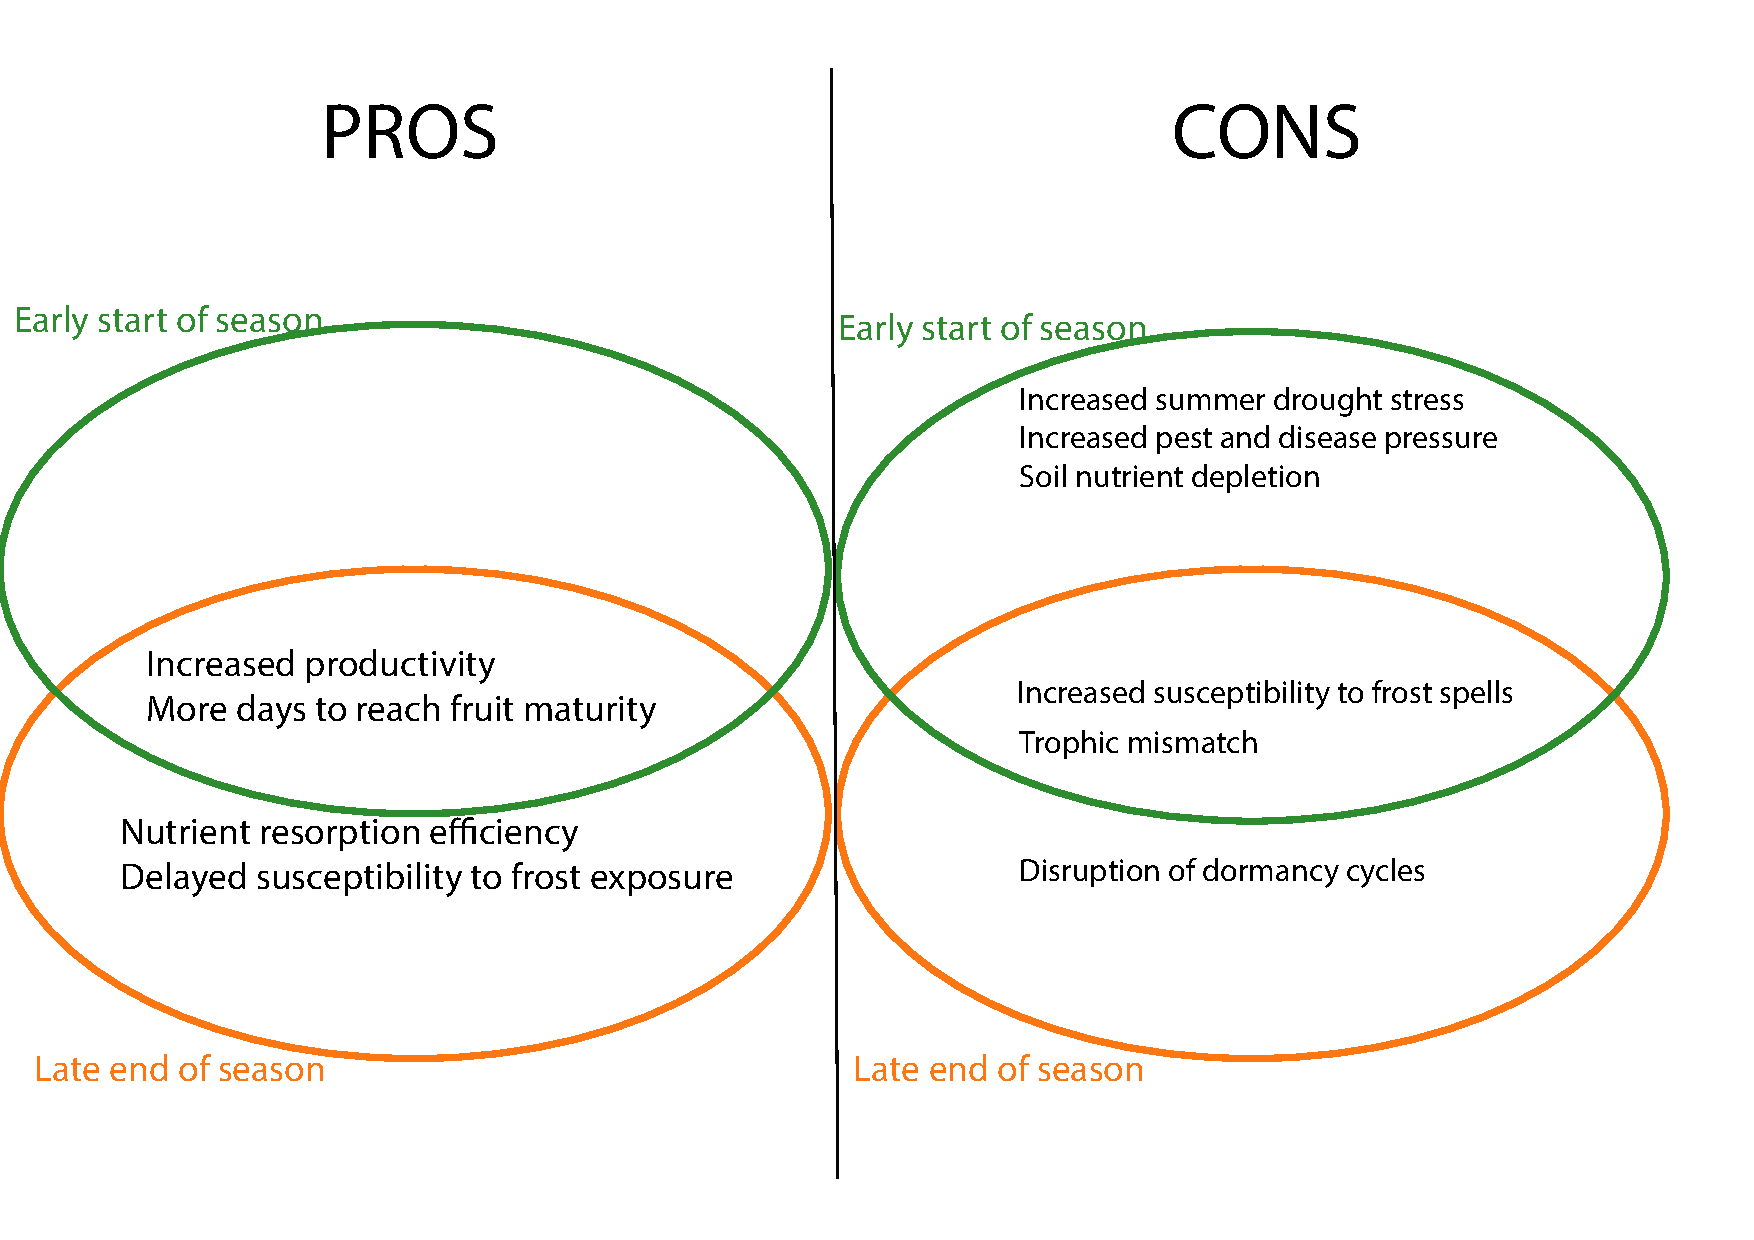
\includegraphics[width=1.1\textwidth]{prosConsFigure.pdf}
\caption{Pros and cons of early start and late end of growing season.}
\label{fig:sample}
\end{figure}

% --- --- --- --- --- --- --- --- --- --- --- --- --- --- --- ---
% References %
% --- --- --- --- --- --- --- --- --- --- --- --- --- --- --- ---

\bibliography{ExportedItems}
\bibliographystyle{ecolett} 

\end{document}
